% ETH Zurich  - 3D Photography 2015
% http://www.cvg.ethz.ch/teaching/3dphoto/
% Template for project proposals

\documentclass[11pt,a4paper,oneside,onecolumn]{IEEEtran}
\usepackage{graphicx}
% Enter the project title and your project supervisor here
\newcommand{\ProjectTitle}{Navigation By Reinforcement Learning}
\newcommand{\ProjectSupervisor}{Nicolay Savinov}
\newcommand{\DateOfReport}{March 9, 2018}

% Enter the team members' names and path to their photos. Comment / uncomment related definitions if the number of members are different than 2.
% Including photographs are optional. Photos are there to help us to evaluate your group more effectively. If you wish not to include your photos, please comment the following line.
\newcommand{\PutPhotos}{}
% Please include a clear photo of each member. (use pdf or png files for Latex to embed them in the document well)
\newcommand{\memberone}{Varin Buff}
\newcommand{\memberonepicture}{pics/buffv}
\newcommand{\membertwo}{Gian Heinrich}
\newcommand{\membertwopicture}{pics/GianAndreaHeinrich}
\newcommand{\memberthree}{Bj\"orn Joos}
\newcommand{\memberthreepicture}{pics/Bjoern}
\newcommand{\memberfour}{Robin St\"ahli}
\newcommand{\memberfourpicture}{pics/Bild_Robin_Staehli}
% \newcommand{\memberfive}{Member Name}
% \newcommand{\memberfivepicture}{pic2.png}


%%%% DO NOT EDIT THE PART BELOW %%%%
\title{\ProjectTitle}
\author{3D Vision Project Proposal\\Supervised by: \ProjectSupervisor\\ \DateOfReport}
\begin{document}
\maketitle
\vspace{-1.5cm}\section*{Group Members}\vspace{0.3cm}
\begin{center}\begin{minipage}{\linewidth}\begin{center}
\begin{minipage}{3 cm}\begin{center}\memberone\ifdefined\PutPhotos\\\vspace{0.2cm}\includegraphics[height=3cm]{\memberonepicture}\fi\end{center}\end{minipage}
\ifdefined\membertwo\begin{minipage}{3 cm}\begin{center}\membertwo\ifdefined\PutPhotos\\\vspace{0.2cm}\includegraphics[height=3cm]{\membertwopicture}\fi\end{center}\end{minipage}\fi
\ifdefined\memberthree\begin{minipage}{3 cm}\begin{center}\memberthree\ifdefined\PutPhotos\\\vspace{0.2cm}\includegraphics[height=3cm]{\memberthreepicture}\fi\end{center}\end{minipage}\fi
\ifdefined\memberfour\begin{minipage}{3 cm}\begin{center}\memberfour\ifdefined\PutPhotos\\\vspace{0.2cm}\includegraphics[height=3cm]{\memberfourpicture}\fi\end{center}\end{minipage}\fi
\ifdefined\memberfive\begin{minipage}{3 cm}\begin{center}\memberfive\ifdefined\PutPhotos\\\vspace{0.2cm}\includegraphics[height=3cm]{\memberfivepicture}\fi\end{center}\end{minipage}\fi
\end{center}\end{minipage}\end{center}\vspace{0.3cm}
%%%% END OF PROTECTED LINES %%%%


%%%% BEGIN WRITING THE DOCUMENT HERE %%%%

\section{Description of the project}

In the Industry 4.0 the need for automation increases tremendously and thus the demand for robots with high navigation abilities in complex three-dimensional surroundings grows vastly. Especially deep learning allows an efficient approach to achieve this. Savinov \textit{et al.} \cite{Nsavinov} used an animal inspired non-metric \cite{Gillner} \cite{Foo} semi-parametric topological memory (SPTM) approach. With this approach, they were able to improve their success rate by a factor of three compared to their baselines. Our team will evaluate further tensorforce based baselines which follow the same evaluation procedure as introduced by Savinov \textit{et al.} \cite{Nsavinov} and will allow to put their work on an even more solid foundation.

\section{Work packages and timeline}

Timeline and project planning
Our project is organized in four main parts. We will start with an orientation phase to gain some knowledge about previously done work, focused mainly on Nikolay Savinovs' paper \cite{Nsavinov}. We will then use our gathered insights to deploy the same environment \cite(GitRepoSavinov) for training and testing of our agent within the vizdoom environment \cite{GitRepoSavinov} and use the same evaluation methods of Reinforcement Learning baselines that were used in \cite{Nsavinov}. We go for this setup to be later able to benchmark the performance of our agent against the results of the paper. 
Our vizdoom agent will be trained with the AC3 algorithm \cite{AC3Ref} and if there is time left also with PPO \cite{PPORef}.
To guarantee an efficient workflow we divide our team into two subgroups, where one team is entrusted with the infrastructural needs of the group, e.g. deploy necessary software on Leonhard. The rest of the group will be focused on the Reinforcement Learning algorithm training and evaluation.
\\

\begin{figure}[htbp] 
	\centering
	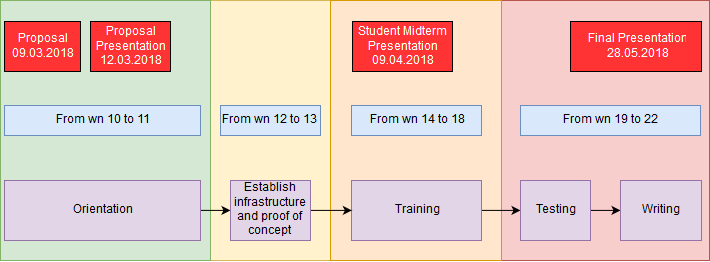
\includegraphics[width=1\textwidth]{pics/ProjectStructure.png}
	\caption{Timeline and project structure}
	\label{fig:timelineprojectstructure}
\end{figure}
We devide those two main tasks into the following subtasks:
\begin{itemize}
	\item Understand previously done work by Nikolay Savinov our Tutor
	\item Utilize interface of Vizdoom envioment
	\item Study Agent movement 
	\item Deploy test program to Leonhard
	\item Prepare midterm presentation
	\item Understand and implement A3C
	\begin{itemize}
		\item Implement rewards and training structure to explore efficiently the maze
		\item Training: we train our agent with the A3C algorithm
		\item Validation: We use the validation mazes to tune our parameters
		\item Testing: testing will be done with the seven provided mazes
	\end{itemize}
	\item If there is time left we implement, train and test our agent with the PPO algorithm additionaly
	\item We compare our results to previous results of Niklay Savinov
	\item Write the final report
\end{itemize}

\section{Outcomes and Demonstration}

The expected outcome of this project is a fully functional agent, implemented with the A3C algorithm and if there is time left the PPO algorithm. Therefore, the agent needs to pass through the same training, validation and testing process as referred to in \cite{Nsavinov}. The performance of said algorithms should be similar or slightly better to the baselines in \cite{NSavinov}, namely in the range of 20\% to 40\% success rate after 5000 steps.
The result will be illustrated as graphs which show the success rate over steps. Furthermore, we want to show the results of the two agents in a demonstration video.


{%\singlespace
{\small
\bibliography{refs}
\bibliographystyle{unsrt}}}

\end{document}